\documentclass{standalone}
\usepackage{xcolor}
\usepackage{tkz-euclide}
\usepackage{calc}
\begin{document}
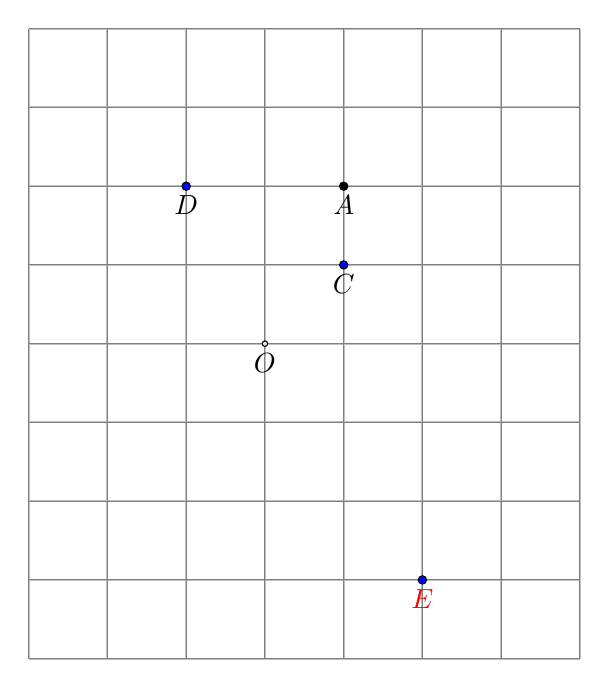
\begin{tikzpicture}
\tkzInit[xmin=-3,xmax=4,ymin=-4,ymax=4]
\tkzGrid[sub,color=gray, subxstep=1,subystep=1]
\tkzAxeXY[very thick]

\coordinate (O) at (0, 0);
\coordinate (A) at (1, 2);

\tkzDefPoint(1,1){C}
\tkzDefPoints{-1/2/D, 2/-3/E}

\tkzDrawPoints(O)
\tkzDrawPoints[size=3, fill=black](A)
\tkzDrawPoints[size=3, fill=blue](C,D,E)

\tkzLabelPoints(O,A,C,D)
\tkzLabelPoints[red](E)


\end{tikzpicture}
\end{document}